
%Chap 3 pag 29
\definecolor{DarkRed}{RGB}{128,0,0}
\definecolor{Green}{RGB}{0,100,0}
\begin{frame}{Implementación: estados vs. nodos}
Un \textcolor{blue}{estado} es una (representación de) una configuración física\\
Un \textcolor{blue}{nodo} es una estructura de datos que constituye parte de un árbol de búsqueda que incluye \textcolor{Green}{padre}, \textcolor{Green}{hijos}, \textcolor{Green}{profundidad}, \textcolor{Green}{costo de ruta} \textcolor{DarkRed}{g(x)}.\\
¡Los estados no tienen padres, hijos, profundidad o costo de ruta!
\begin{figure}
    \centering
    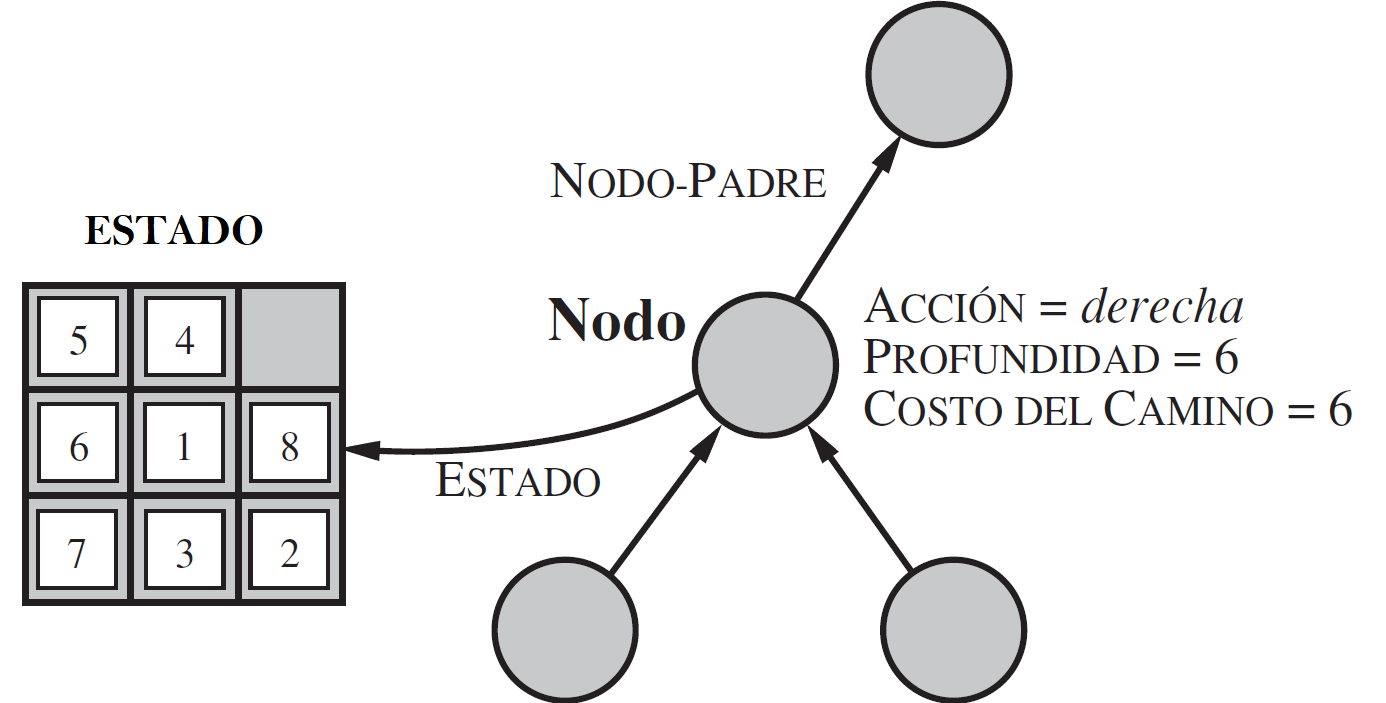
\includegraphics[width = 60mm, scale = 0.7]{images/29_image.PNG}
\end{figure}
La función \rmfamily{\textit{Expand}} crea nuevos nodos, completando los diversos campos\\
\hspace{0.8cm}y usando el \rmfamily{\textit{SuccessorFn}} del problema para crear los\\
\hspace{0.8cm}estados correspondientes.
\end{frame}
